\section{Polymorphie}


{\setbeamertemplate{footline}{\parbox{\linewidth}{\vspace*{-8pt}Quelle: \url{https://de.wikipedia.org/wiki/Polymorphie_(Programmierung)}}}
\begin{frame}
	\frametitle{Polymorphie}
	\begin{itemize}
		\item wird auch Vielgestaltigkeit oder Polymorphismus genannt
		\item Gleiches Interface für Objekte von verschiedenen Typen
		\item Ein Bezeichner kann Objekte unterschiedlicher Typen annehmen
		\item Gegenteil: Monomorphie
	\end{itemize}
	\begin{table}[h]
	\begin{tabularx}{\textwidth}{$l|^X|^X}
		\rowstyle{\bfseries}  & universell                              & ad-hoc                             \\
		\rowstyle{\small}     & unendlich viele Typen                   & endliche Anzahl an Typen           \\
		\rowstyle{\small}     & eine Implementierung                    & unterschiedliche Implementierungen \\
		\hline
		\bfseries dynamisch   & \multirow{2}{*}{Inklusionspolymorphie/} &                                    \\
		\small    Laufzeit    & \multirow{2}{*}{Vererbungspolymorphie}  &                                    \\
		\small    langsamer   &                                         &                                    \\
		\hline
		\bfseries statisch    & \multirow{2}{*}{parametrische}          & \multirow{2}{*}{Überladung,}        \\
		\small    Kompilezeit & \multirow{2}{*}{Polymorphie}            & \multirow{2}{*}{Coercion}          \\
		\small    schneller   &                                         &                                    \\
	\end{tabularx}
\end{table}

\end{frame}
}

{\setbeamertemplate{footline}{\parbox{\linewidth}{\vspace*{-8pt}Quelle: \url{https://de.wikipedia.org/wiki/Polymorphie_(Programmierung)\#Universelle_und_Ad-hoc-Polymorphie}}}
\begin{frame}
	\frametitle{universelle Polymorphie}
	\begin{itemize}
		\item Gleiches Interface für unendlich viele Typen
		\item Eine Implementierung
		\item ``echte Vielgestaltigkeit''
		\item Unterarten:
		\begin{itemize}
			\item Inklusionspolymorphie
			\item Vererbungspolymorphie
			\item Parametrische Polymorphie
		\end{itemize}
	\end{itemize}
\end{frame}
}


{\setbeamertemplate{footline}{\parbox{\linewidth}{\vspace*{-8pt}Quelle: \url{https://en.wikipedia.org/wiki/Subtyping}}}
\begin{frame}
	\frametitle{Inklusionspolymorphie}
	\begin{itemize}
		\item Liskovsches Substitutionsprinzip ist erfüllt
		\begin{itemize}
			\item Objekt des Typ A kann problemlos, durch Objekt des Typ B ersetzt werden, ohne dass sich das Verhalten ändert
		\end{itemize}
	\end{itemize}
\end{frame}
}

{\setbeamertemplate{footline}{\parbox{\linewidth}{\vspace*{-8pt}Quelle: \url{https://de.wikipedia.org/wiki/Vererbung_(Programmierung)}}}
\begin{frame}
	\frametitle{Vererbungspolymorphie}
	\begin{itemize}
		\item Dynamisch
		\item Kann Inklusionspolymorphie ausdrücken
		\item Sollte auch das Liskovsche Substitutionsprinzip befolgen, muss aber nicht
		\item Virtuelle Methoden
	\end{itemize}
\end{frame}
}

{\setbeamertemplate{footline}{\parbox{\linewidth}{\vspace*{-8pt}Vollständiges Beispiel: \url{https://godbolt.org/z/WaG3z5s4d}}}
\begin{frame}
	\frametitle{Beispiel -- Fahrzeug: Mehrfache Auswahl}
	{\tiny\UseRawInputEncoding{\lstinputlisting[language={C++}]{polymorphie/universell/vererbung/beispiele/fahrzeug/fahrzeug.bad.cpp}}\inputencoding{utf8}}
\end{frame}
}

{\setbeamertemplate{footline}{\parbox{\linewidth}{\vspace*{-8pt}Vollständiges Beispiel: \url{https://godbolt.org/z/zx4jqErf6}}}
\begin{frame}
	\frametitle{Beispiel -- Fahrzeug: Vererbungspolymorphie}
	{\tiny\UseRawInputEncoding{\lstinputlisting[language={C++}]{polymorphie/universell/vererbung/beispiele/fahrzeug/fahrzeug.good.cpp}}\inputencoding{utf8}}
\end{frame}
}

{\setbeamertemplate{footline}{\parbox{\linewidth}{\vspace*{-8pt}Vollständiger Code: \url{https://github.com/PaulRaffer/Snake}}}
\begin{frame}
	\frametitle{Beispiel -- Snake}
	\begin{figure}[H]
		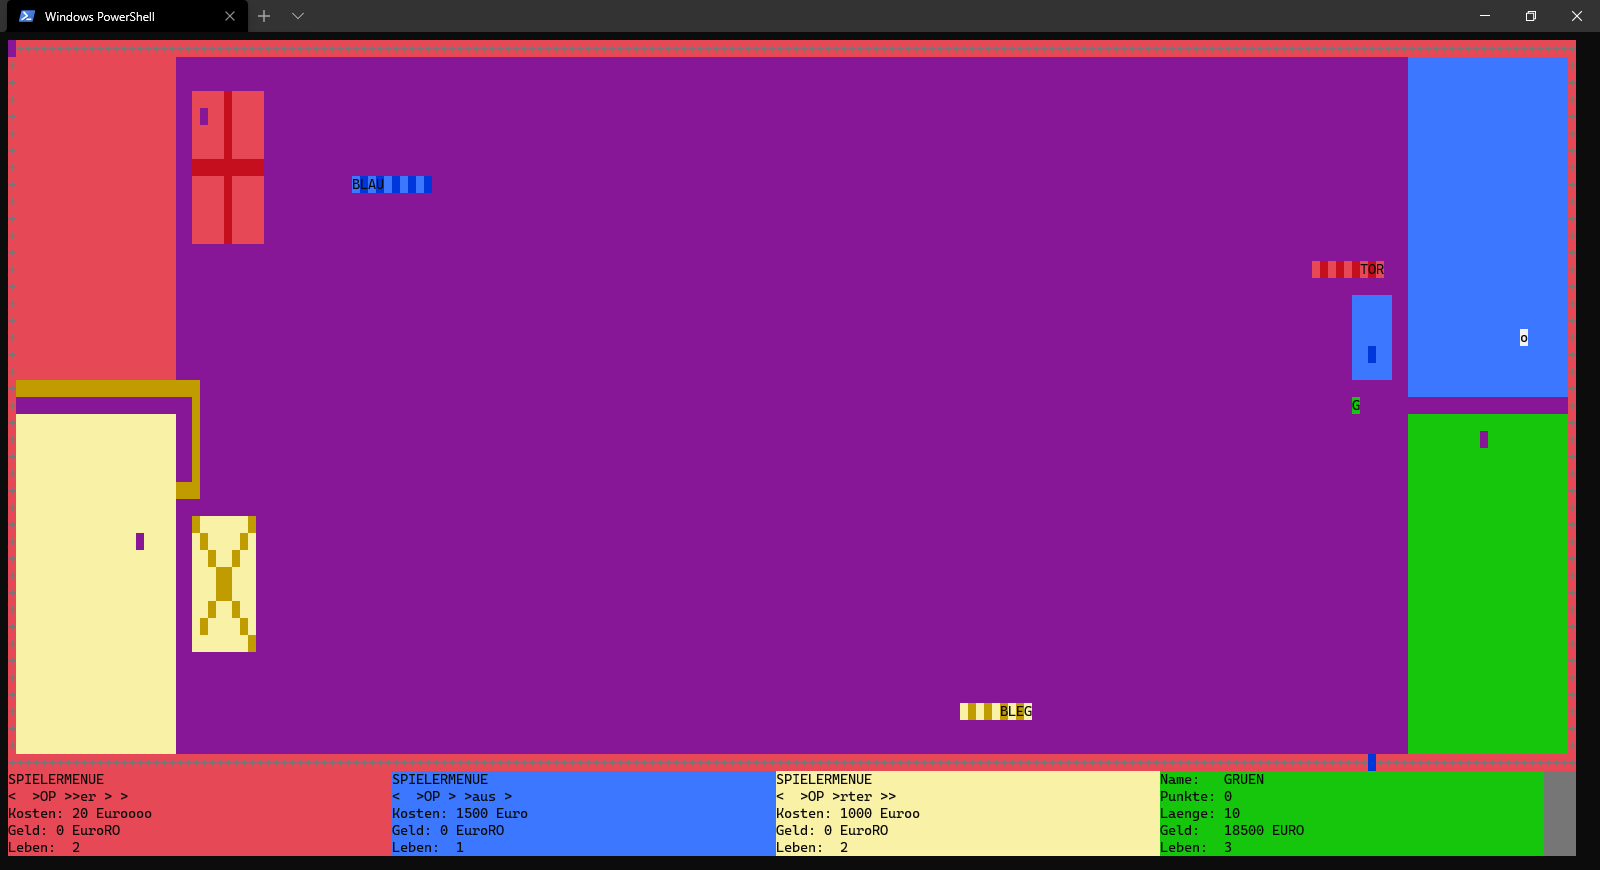
\includegraphics[width=\textwidth]{polymorphie/universell/vererbung/beispiele/snake/snake.png}
	\end{figure}
\end{frame}
}

{\setbeamertemplate{footline}{\parbox{\linewidth}{\vspace*{-8pt}Vollständiger Code: \url{https://github.com/PaulRaffer/Snake}}}
\begin{frame}
	\frametitle{Beispiel -- Snake}
	\begin{itemize}
		\item Unterschiedliche Arten von Gebäuden (Kanonen, Mauern, Geldlager, Krankenhäuser, ...)
		\item Unterschiedliche Arten von Punkten (normale Punkte, Geld, Leben, ...)
	\end{itemize}
\end{frame}
}

{\setbeamertemplate{footline}{\parbox{\linewidth}{\vspace*{-8pt}Vollständiger Code: \url{https://github.com/PaulRaffer/Snake}}}
\begin{frame}[t]
	\frametitle{Beispiel -- Snake: Mein Code (nicht nachmachen!)}
	{\tiny\UseRawInputEncoding{\lstinputlisting[language={C++}]{polymorphie/universell/vererbung/beispiele/snake/snake_gebaeude.bad.cpp}}\inputencoding{utf8}}
\end{frame}
}

{\setbeamertemplate{footline}{\parbox{\linewidth}{\vspace*{-8pt}Vollständiger Code: \url{https://github.com/PaulRaffer/Snake}}}
\begin{frame}[t]
	\frametitle{Beispiel -- Snake: Vererbungspolymorphie}
	\begin{figure}[H]
		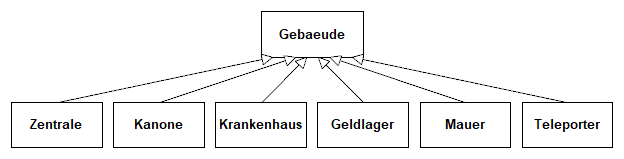
\includegraphics[width=\textwidth]{polymorphie/universell/vererbung/beispiele/snake/gebaeude.png}
	\end{figure}
	{\tiny\UseRawInputEncoding{\lstinputlisting[language={C++}]{polymorphie/universell/vererbung/beispiele/snake/snake_gebaeude.good.cpp}}\inputencoding{utf8}}
\end{frame}
}

{\setbeamertemplate{footline}{\parbox{\linewidth}{\vspace*{-8pt}Quelle: \url{https://de.wikipedia.org/wiki/Kreis-Ellipse-Problem}}}
\begin{frame}
	\frametitle{Kreis-Ellipse-Problem}
	\begin{itemize}
		\item Problem:
		\begin{itemize}
			\item Basisklasse 'Form' hat die Methoden 'zeichnen' und 'flaeche'
			\item Ellipsen und Kreise sollen erstellt werden können
			\item 'Kreis' erbt von 'Ellipse' erbt von 'Form'
			\item Es gibt die Setter 'set\_x' und 'set\_y' zum skalieren
			\item Bei Kreisen können nicht beide Dimensionen unabhängig voneinander skaliert werden
			\item Liskovsches Substitutionsprinzip nicht erfüllt
		\end{itemize}
		
		\item Lösungsvorschläge:
		\begin{itemize}
			\item Fehler bei Größenänderung
			\item 'Ellipse' erbt von 'Kreis'
			\item Keine Klasse 'Kreis'
			\item Keine Vererbungsbeziehung zwischen 'Ellipse' und 'Kreis'
			\item Einführen neuer Basisklasse
		\end{itemize}
		
		\item Keiner der Lösungsvorschläge ist ideal
		\item Nicht jede ``ist-ein''-Beziehung sollte durch öffentliche Vererbung dargestellt werden!
	\end{itemize}
\end{frame}
}


{\setbeamertemplate{footline}{\parbox{\linewidth}{\vspace*{-8pt}Quelle: \url{https://soundcloud.com/lambda-cast/9-polymorphism-and-abstraction}}}
\begin{frame}
	\frametitle{Parametrische Polymorphie}
	\begin{itemize}
		\item Vor allem in funktionalen Sprachen verbreitet
		\item Algorithmen bzw. Klassen werden allgemein beschrieben, damit sie mit Objekten unterschiedlicher Typen funktionieren
		\item Generics, Templates, ...
	\end{itemize}
\end{frame}
}


{\setbeamertemplate{footline}{\parbox{\linewidth}{\vspace*{-8pt}Quelle: \url{https://en.wikipedia.org/wiki/Ad_hoc_polymorphism}}}
\begin{frame}
	\frametitle{Ad-hoc-Polymorphie}
	\begin{itemize}
		\item Gleiche Schnittstelle für begrenzte Anzahl an bestimmten Typen
		\item Eine Implementierung pro Typ
		\item Unterarten:
		\begin{itemize}
			\item Coercion
			\item Überladung
		\end{itemize}
	\end{itemize}
\end{frame}
}

{\setbeamertemplate{footline}{\parbox{\linewidth}{\vspace*{-8pt}Quelle: \url{https://de.wikipedia.org/wiki/\%C3\%9Cberladen}}}
\begin{frame}
	\frametitle{Überladung}
	\begin{itemize}
		\item Statisch
		\item Mehrere Funktionen haben den gleichen Namen
		\item Operatorüberladung
	\end{itemize}
	{\scriptsize\bfseries C:}
		{\tiny\UseRawInputEncoding{\lstinputlisting[language={C++}]{polymorphie/adhoc/ueberladung/beispiele/print/print.c}}\inputencoding{utf8}}
	{\scriptsize\bfseries C++:}
		{\tiny\UseRawInputEncoding{\lstinputlisting[language={C++}]{polymorphie/adhoc/ueberladung/beispiele/print/print.cpp}}\inputencoding{utf8}}
\end{frame}
}

{\setbeamertemplate{footline}{\parbox{\linewidth}{\vspace*{-8pt}Quelle: \url{https://en.wikipedia.org/wiki/Type_conversion}}}
\begin{frame}
	\frametitle{Coercion}
	\begin{itemize}
		\item Statisch
		\item Implizite Typumwandlung
	\end{itemize}
	{\tiny\UseRawInputEncoding{\lstinputlisting[language={C++}]{polymorphie/adhoc/coercion/beispiele/src/eingebauteDatentypen.cpp}}\inputencoding{utf8}}
\end{frame}
}

{\setbeamertemplate{footline}{\parbox{\linewidth}{\vspace*{-8pt}Quelle: Grundkurs C++}}
\begin{frame}
	\frametitle{Coercion - Konvertierungskonstruktor (C++)}
	{\tiny\UseRawInputEncoding{\lstinputlisting[language={C++}]{polymorphie/adhoc/coercion/beispiele/src/konvertierungskonstruktoren.cpp}}\inputencoding{utf8}}
\end{frame}
}

{\setbeamertemplate{footline}{\parbox{\linewidth}{\vspace*{-8pt}Quelle: Grundkurs C++}}
\begin{frame}
	\frametitle{Coercion - Konvertierungsoperator (C++)}
	{\tiny\UseRawInputEncoding{\lstinputlisting[language={C++}]{polymorphie/adhoc/coercion/beispiele/src/konvertierungsoperatoren.cpp}}\inputencoding{utf8}}
\end{frame}
}
